\documentclass[conference]{IEEEtran}
\IEEEoverridecommandlockouts
% The preceding line is only needed to identify funding in the first footnote. If that is unneeded, please comment it out.
%Template version as of 6/27/2024

\usepackage{cite}
\usepackage{amsmath,amssymb,amsfonts}
\usepackage{algorithmic}
\usepackage{graphicx}
\usepackage{textcomp}
\usepackage{xcolor}

\usepackage{float} 
\usepackage{placeins}

\usepackage{colortbl}  % Required for \rowcolor
\usepackage{xcolor}    % Provides additional color definitions

% Digunakan untuk menampilkan pustaka.
\usepackage[square,comma,numbers,sort&compress]{natbib}

% Mengubah format ukuran teks pada natbib.
\renewcommand{\bibfont}{\normalfont\footnotesize}

% Digunakan untuk menyeimbangkan bagian akhir dokumen dengan dua kolom.
\usepackage{balance}

\def\BibTeX{{\rm B\kern-.05em{\sc i\kern-.025em b}\kern-.08em
    T\kern-.1667em\lower.7ex\hbox{E}\kern-.125emX}}
\begin{document}

\title{AUTONOMOUS VEHICLE NAVIGATION SYSTEM USING MACHINE LEARNING AND GRAPH BASED SLAM
}

\author{\IEEEauthorblockN{Azzam Wildan Maulana}
\IEEEauthorblockA{\textit{Departemen of Electrical Engineering} \\
\textit{Faculty of Intelligent Electrical and Informatics Technolog} \\
\textit{Sepuluh Nopember Institute of Technology}\\
Surabaya, Indonesia \\
azzamwildan462@gmail.com}
\and

\IEEEauthorblockN{Rudy Dikairono}
\IEEEauthorblockA{Department of Electrical Engineering\\
Faculty of Intelligent Electrical and Informatics Technology\\
Institut Teknologi Sepuluh Nopember\\
Surabaya, Indonesia 60111\\
rudydikairono@its.ac.id}
\and

\IEEEauthorblockN{Ahmad Zaini}
\IEEEauthorblockA{Department of Computer Engineering\\
Faculty of Intelligent Electrical and Informatics Technology\\
Institut Teknologi Sepuluh Nopember\\
Surabaya, Indonesia 60111\\
zaini@its.ac.id}
\and

\IEEEauthorblockN{Mauridhi Hery Purnomo}
\IEEEauthorblockA{\textit{Departemen of Computer Engineering} \\
\textit{Faculty of Intelligent Electrical and Informatics Technolog} \\
\textit{Sepuluh Nopember Institute of Technology}\\
Surabaya, Indonesia \\
hery@ee.its.ac.id}
\and
}

\maketitle

\begin{abstract}
	Icar is an autonomous vehicle developed by Institut Teknologi Sepuluh Nopember (ITS) to autonomously navigate the campus environment. Its navigation system relies on pose estimation using sensor fusion between odometry and the Global Navigation Satellite System (GNSS). However, GNSS signals are prone to degradation in environments with obstacles such as tall buildings and trees, while odometry suffers from inaccuracies caused by wheel slippage, encoder drift, and inertial sensor errors. These limitations result in unreliable localization, potentially causing Icar to deviate from its designated trajectory.

	To address these issues, this research proposes an enhanced navigation system by integrating a stereo depth camera and LIDAR. Road detection is performed using a semantic segmentation model based on deep learning, enabling Icar to distinguish road surfaces from non-road areas. Pose refinement is carried out using graph-based optimization within a SLAM framework, incorporating data from the depth camera and LIDAR processed via the Iterative Closest Point (ICP) algorithm. The proposed system improves localization robustness and offers a GNSS-independent alternative for safe and accurate autonomous navigation. The final system is expected to reduce dependency on GNSS and increase Icar's reliability in semi-structured or dynamic environments.
\end{abstract}

\begin{IEEEkeywords}
	Autonomous vehicle, Icar, GNSS, Odometry, Pose Estimation, Stereo Depth Camera, Semantic Segmentation, SLAM, ICP, Graph-Based Optimization, Deep Learning
\end{IEEEkeywords}


\section{Background}
Icar is an autonomous vehicle developed by Institut Teknologi Sepuluh Nopember (ITS). Icar is designed to operate automatically and navigate throughout the ITS campus. Its control system relies on pose estimation (i.e., position and orientation) derived from odometry and sensor fusion with the Global Navigation Satellite System (GNSS). The estimated pose is then used to guide Icar toward a predetermined destination.

\par
The pose of Icar is determined through the combination of odometry and GNSS data. Odometry estimates pose based on wheel rotations, augmented by a gyroscope to obtain orientation. GNSS, on the other hand, estimates pose based on satellite signals. These two sources are fused using the Extended Kalman Filter algorithm to achieve higher accuracy in pose estimation \cite{ref_mas_marin}.

\par 
However, the data provided by GNSS is not always fully reliable. Several environmental conditions, such as tall buildings or dense tree canopies, can obstruct satellite signals. This may cause a phenomenon known as multipath, in which satellite signals reach the receiver via multiple indirect paths, resulting in errors in position and orientation estimation \cite{ref_gnss_multipath}.

\par 
Errors can also arise from the odometry system due to factors such as inaccurate wheel travel distance, incorrect wheel rotation angle calculations, or faulty IMU sensor readings. These inaccuracies may result from differences in wheel diameters, uneven tire pressure, or wheel slippage. Moreover, errors in wheel rotation angle measurements may originate from malfunctioning encoder sensors \cite{ref_odom_error}.

\par
When errors occur in pose estimation, Icar may deviate from its intended trajectory. This can lead to safety concerns, such as collisions with obstacles or deviation from designated transportation lanes. Therefore, an additional navigation system is required to enhance pose accuracy and ensure safe autonomous navigation.

\par
A promising enhancement is the integration of a stereo depth camera, which provides visual depth information to detect roads. This road detection process employs a machine learning algorithm—specifically, semantic segmentation—trained on labeled datasets to distinguish between road and non-road areas \cite{ref_mas_pandu}.

\par 
Beyond road detection, the stereo depth camera is also used to refine pose estimation through graph-based optimization. Furthermore, a LIDAR sensor is incorporated and processed using the Iterative Closest Point (ICP) algorithm to further improve localization accuracy. Together, these methods form a Simultaneous Localization and Mapping (SLAM) system \cite{thrun2005probabilistic}, which is expected to potentially replace the role of GNSS entirely.

% =========================================================================================================

\section{Literature Review}
There are several studies to dive deeper into the topic of autonomous vehicle navigation systems. These studies focus on various aspects, including pose estimation, road detection, and SLAM implementation.

\subsection{Odometry}
Odometry is an algorithm used to estimate how far a robot has traveled. In a 2D pose system, the robot’s movement is represented as \(x, y, \text{yaw}\). The simplest form of 2D odometry combines motor rotation data with orientation data from an Inertial Measurement Unit (IMU). By applying forward kinematics to this sensor data, the robot's pose can be estimated relative to its initial position \cite{ref_mas_marin}.

\subsection{Kalman Filter}
The Kalman Filter is a powerful linear estimation algorithm used to predict and update the state of dynamic systems based on noisy sensor data. Introduced by Rudolf E. Kalman in 1960, it enables accurate real-time estimation of variables such as position and velocity \cite{kalman1960new}. In robotics and control systems, the Kalman Filter is instrumental in fusing data from multiple sensors such as GNSS, IMUs, and wheel encoders.

\subsection{Semantic Segmentation}

Fast-SCNN (Fast Semantic Segmentation Convolutional Neural Network) was designed for real-time performance on resource-constrained devices, making it ideal for embedded systems like autonomous vehicles. It combines a lightweight encoder-decoder structure with efficient components such as depthwise separable convolutions and a streamlined feature fusion strategy. These design choices enable Fast-SCNN to achieve a good balance between accuracy and speed, ensuring that road segmentation can be performed in real time without requiring GPU-level hardware.

\begin{figure}[H]
	\centering
	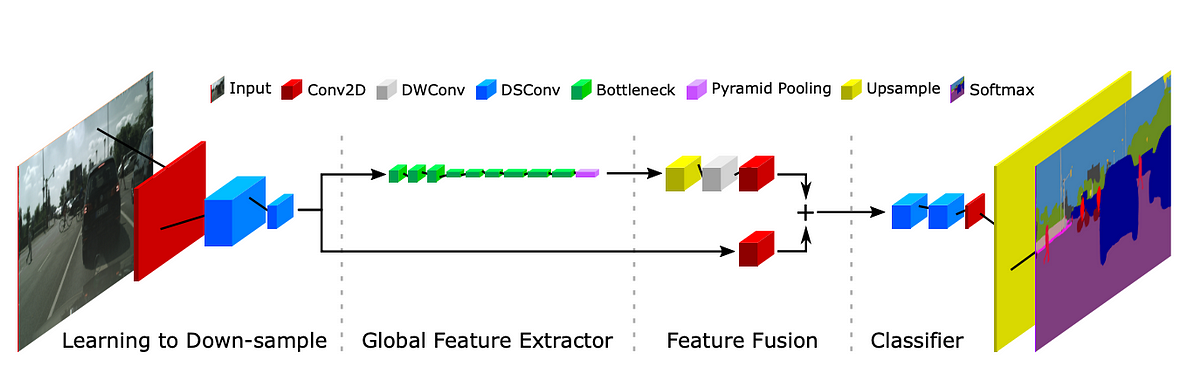
\includegraphics[width=\linewidth]{../konten/fast_scnn.png}
	\caption{Fast SCNN Architecture \cite{ref_fast_scnn}}
	\label{fig:fast_scnn_architecture}
\end{figure} 

Fast-SCNN consists of four main modules: Learning to Downsample, Global Feature Extractor, Feature Fusion Module, and Classifier. The network first reduces the spatial dimensions of the input image while increasing feature richness, then extracts global context features and fuses them with fine spatial details. This fused representation is finally classified at the pixel level to distinguish road and non-road areas. In the Icar system, this segmented output supports safe navigation by identifying drivable regions based on real-time camera input \cite{ref_fast_scnn}.


\subsection{Graph-Based SLAM}
SLAM techniques can be divided into two broad categories: filter-based SLAM (e.g., Extended Kalman Filter SLAM) and graph-based SLAM. In filter-based SLAM, the robot's pose and landmark positions are treated as stochastic variables updated recursively. In contrast, graph-based SLAM builds a graph where nodes represent robot poses and landmarks, and edges represent spatial constraints derived from sensor observations \cite{thrun2005probabilistic}.

\begin{figure}[H]
	\centering
	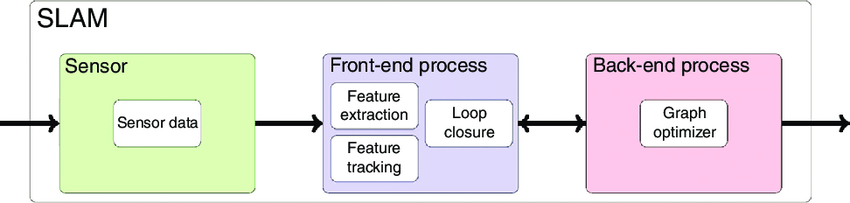
\includegraphics[width=\linewidth]{../konten/gb_slam.png}
	\caption{Basic Graph-Based SLAM Architecture \cite{ref_gb_slam}}
	\label{fig:basic_graph_based_slam}
\end{figure} 

There are three main process that can be seen from figure \ref{fig:basic_graph_based_slam}: The first process is sensor data, it means like acquiring data from sensors such as cameras, LIDAR, or IMU. The second process is front end process, The front end process is responsible for extracting features from the sensor data and finding a loop closure. The last process is back end process, the back end process is responsible for optimizing the graph to find the best estimate of the robot's trajectory and the map of the environment \cite{ref_gb_slam}.

\par
The optimization in Graph-based SLAM can be efficiently implemented using frameworks like GTSAM (Georgia Tech Smoothing and Mapping), a C++ library that applies nonlinear optimization over factor graphs. Factor graphs represent probabilistic relationships among variables such as odometry, landmarks, and sensor observations, and allow for efficient optimization of robot trajectories \cite{ref_gtsam}.

\subsection{Bicycle Model}
The bicycle model is a simplified mathematical representation of vehicle dynamics. It models a vehicle as a two-wheel system—one at the front and one at the rear—mimicking the dynamics of a bicycle. This model is widely used in vehicle control and trajectory planning due to its simplicity and ability to capture basic vehicle behavior \cite{rajamani2011vehicle}. In robotics and electrical engineering, the bicycle model is commonly used to develop navigation and motion control algorithms for autonomous ground vehicles.

\begin{equation}
	\begin{aligned}
		\delta_{\text{target}} &= \tan^{-1}\left( \frac{2 \cdot L \cdot \sin(\theta_{\text{direction}})}{D_{\text{lookahead}}} \right)
		\label{eq:bicycle_model_core}
	\end{aligned}		
\end{equation}

where \(\delta_{\text{target}}\) is the target steering angle, \(L\) is the distance between the front and rear wheels, \(\theta_{\text{direction}}\) is the heading angle, and \(D_{\text{lookahead}}\) is the lookahead distance.

\par
The main advantage of the bicycle model is its applicability in control and simulation algorithms such as PID, LQR, and MPC. Many autonomous vehicle systems use it as a foundational model for motion prediction and path following. For instance, it enables calculation of the optimal steering angle required for a vehicle to accurately and stably follow a predefined trajectory \cite{paden2016survey}.

% =========================================================================================================

\section{Methodology}
There are some proposed methods to improve the navigation system of Icar. 

\subsection{Overview of the Icar System} 
The navigation system in Icar is divided into two types: the legacy navigation system using GNSS and the new navigation system that operates without GNSS. Below are block diagrams of Icar's navigation systems with and without GNSS.

\begin{figure}[H]
	\centering
	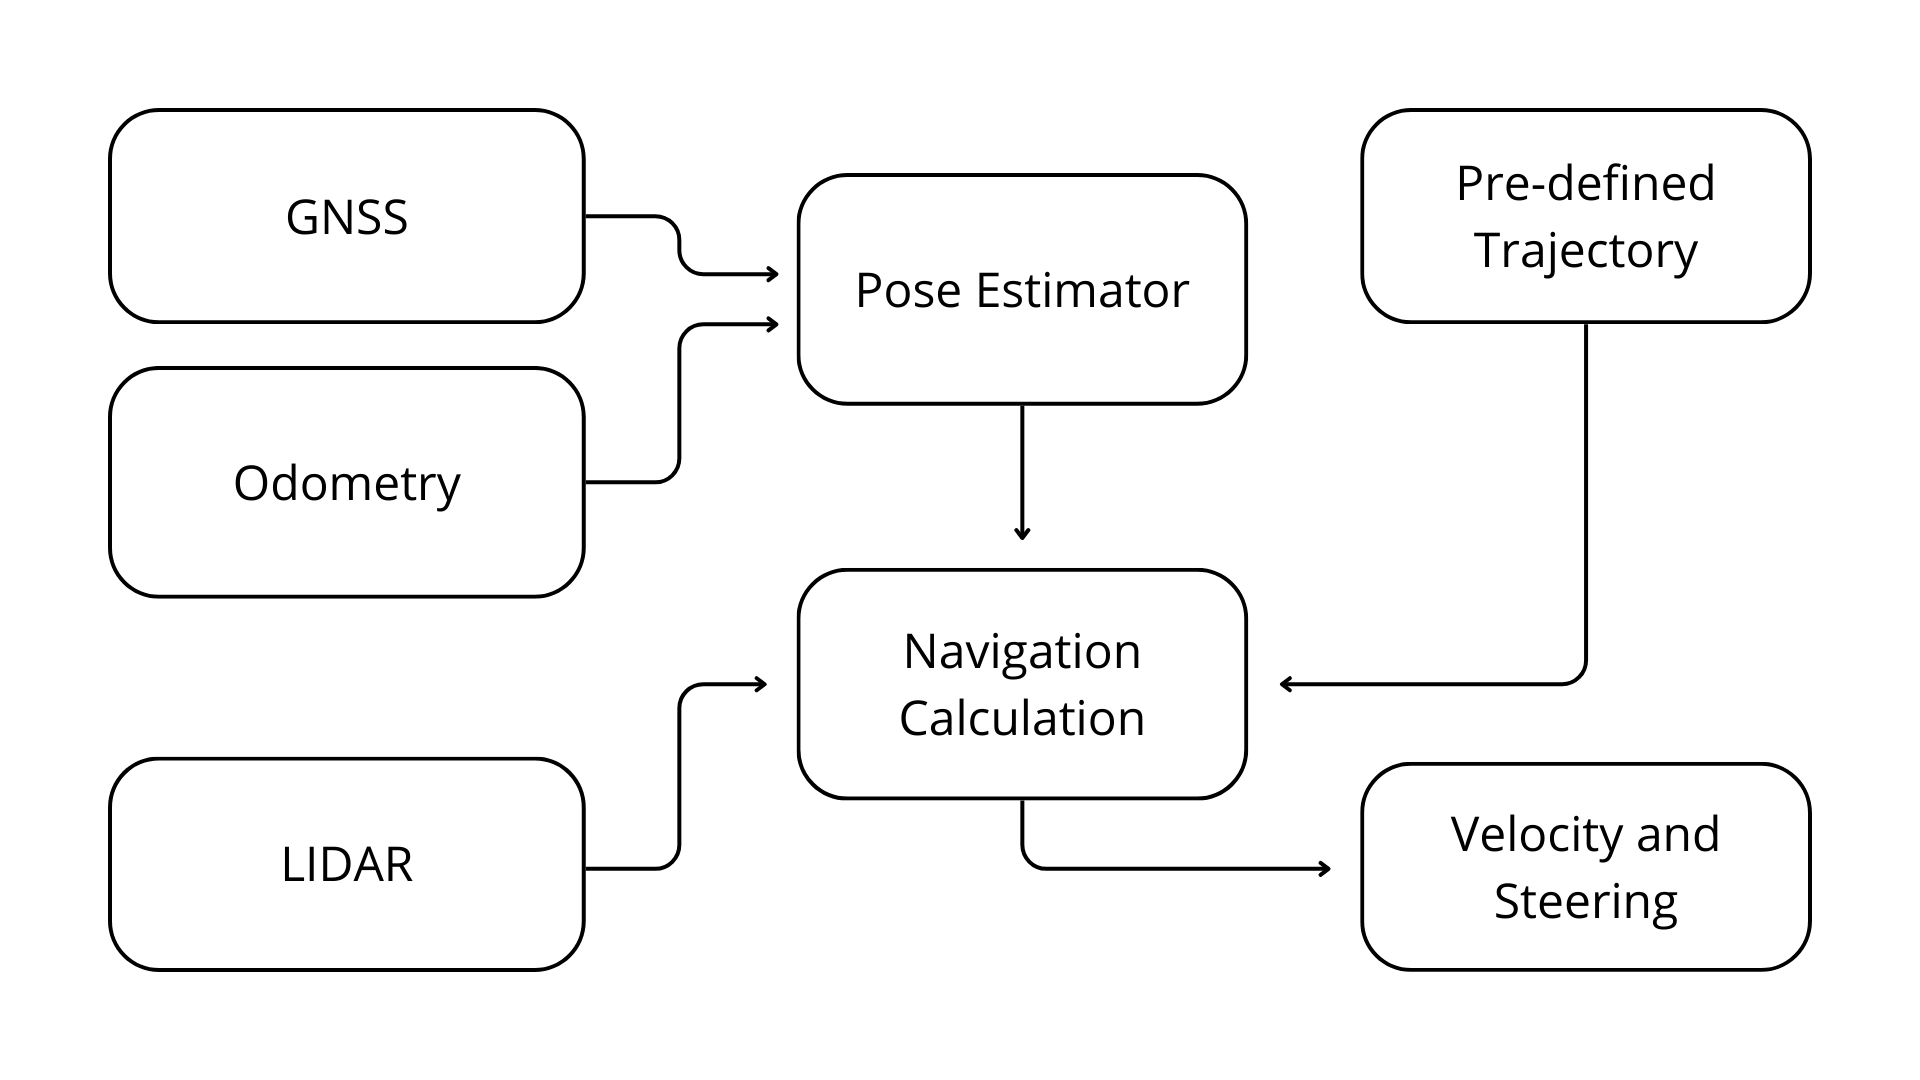
\includegraphics[width=\linewidth]{../konten/full_sys1.png}
	\caption{Block Diagram of the Legacy Icar System with GNSS}
	\label{fig:full_system}
\end{figure}
\FloatBarrier

Figure \ref{fig:full_system} illustrates the legacy Icar system, which relies on GNSS and odometry for pose estimation. The system uses a Pre-defined Trajectory to determine the target speed and steering angle using the Bicycle Model, as shown in equation~\ref{eq:bicycle_model_core}.

\begin{figure}[H]
	\centering
	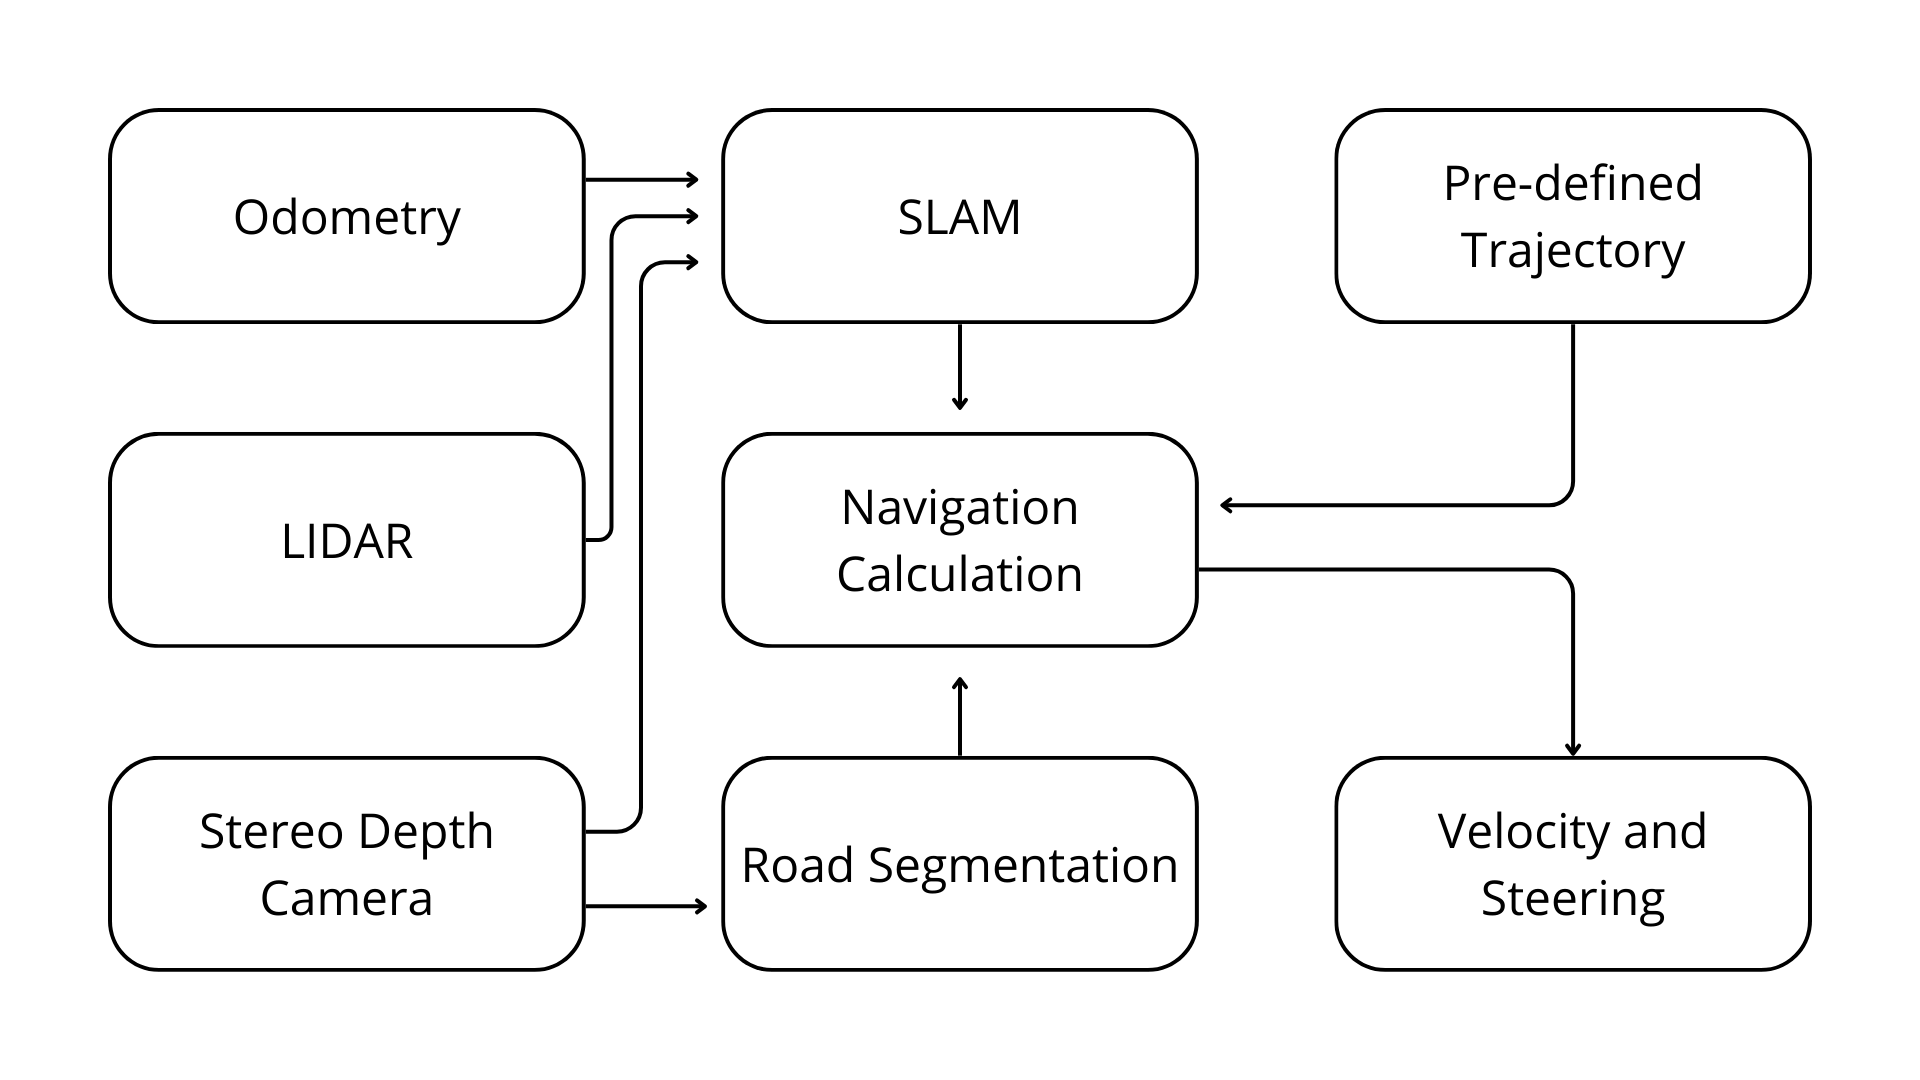
\includegraphics[width=\linewidth]{../konten/full_sys_slam1.png}
	\caption{Block Diagram of the New Icar System without GNSS}
	\label{fig:full_system_slam}
\end{figure}

Figure \ref{fig:full_system_slam} illustrates the new proposed Icar system, which does not rely on GNSS. Instead, it uses a stereo depth camera and LIDAR for pose estimation. The system also employs a Pre-defined Trajectory to determine the target speed and steering angle using the Bicycle Model, as shown in equation~\ref{eq:bicycle_model_full}. Below is the full equation for the Bicycle Model used in the new system:

\begin{equation}
	\begin{aligned}
		\Delta x &= x_{\text{waypoint}} - x_{\text{position}} \\
		\Delta y &= y_{\text{waypoint}} - y_{\text{position}} \\
		\theta_{\text{direction}} &= \tan^{-1}\left(\frac{\Delta y}{\Delta x}\right) - \theta_{\text{orientation}} \\
		v_{\text{target}} &= \min\left(\sqrt{\Delta x^2 + \Delta y^2}, \ v_{\text{max}}\right) \\
		\delta_{\text{target}} &= \tan^{-1}\left( \frac{2 \cdot L \cdot \sin(\theta_{\text{direction}})}{D_{\text{lookahead}}} \right)
		\label{eq:bicycle_model_full}
	\end{aligned}		
\end{equation}

Where $x_{\text{waypoint}}$ and $y_{\text{waypoint}}$ are the coordinates of the waypoint obtained from the Pre-defined Trajectory, $x_{\text{position}}$ and $y_{\text{position}}$ represent the vehicle's current position, $\theta_{\text{direction}}$ is the heading angle, $\theta_{\text{orientation}}$ is the current orientation, $v_{\text{target}}$ is the target velocity, $v_{\text{max}}$ is the maximum velocity, $\delta_{\text{target}}$ is the target steering angle, $L$ is the distance between the front and rear wheels, and $D_{\text{lookahead}}$ is the lookahead distance.

The primary difference between the two systems is the source of position and orientation data. The legacy system uses GNSS and odometry, while the new system uses stereo depth cameras, LIDAR, and odometry. Additionally, the new system integrates road detection to enhance navigation safety.

\subsection{Road Detection System}
\begin{figure}[H]
	\centering
	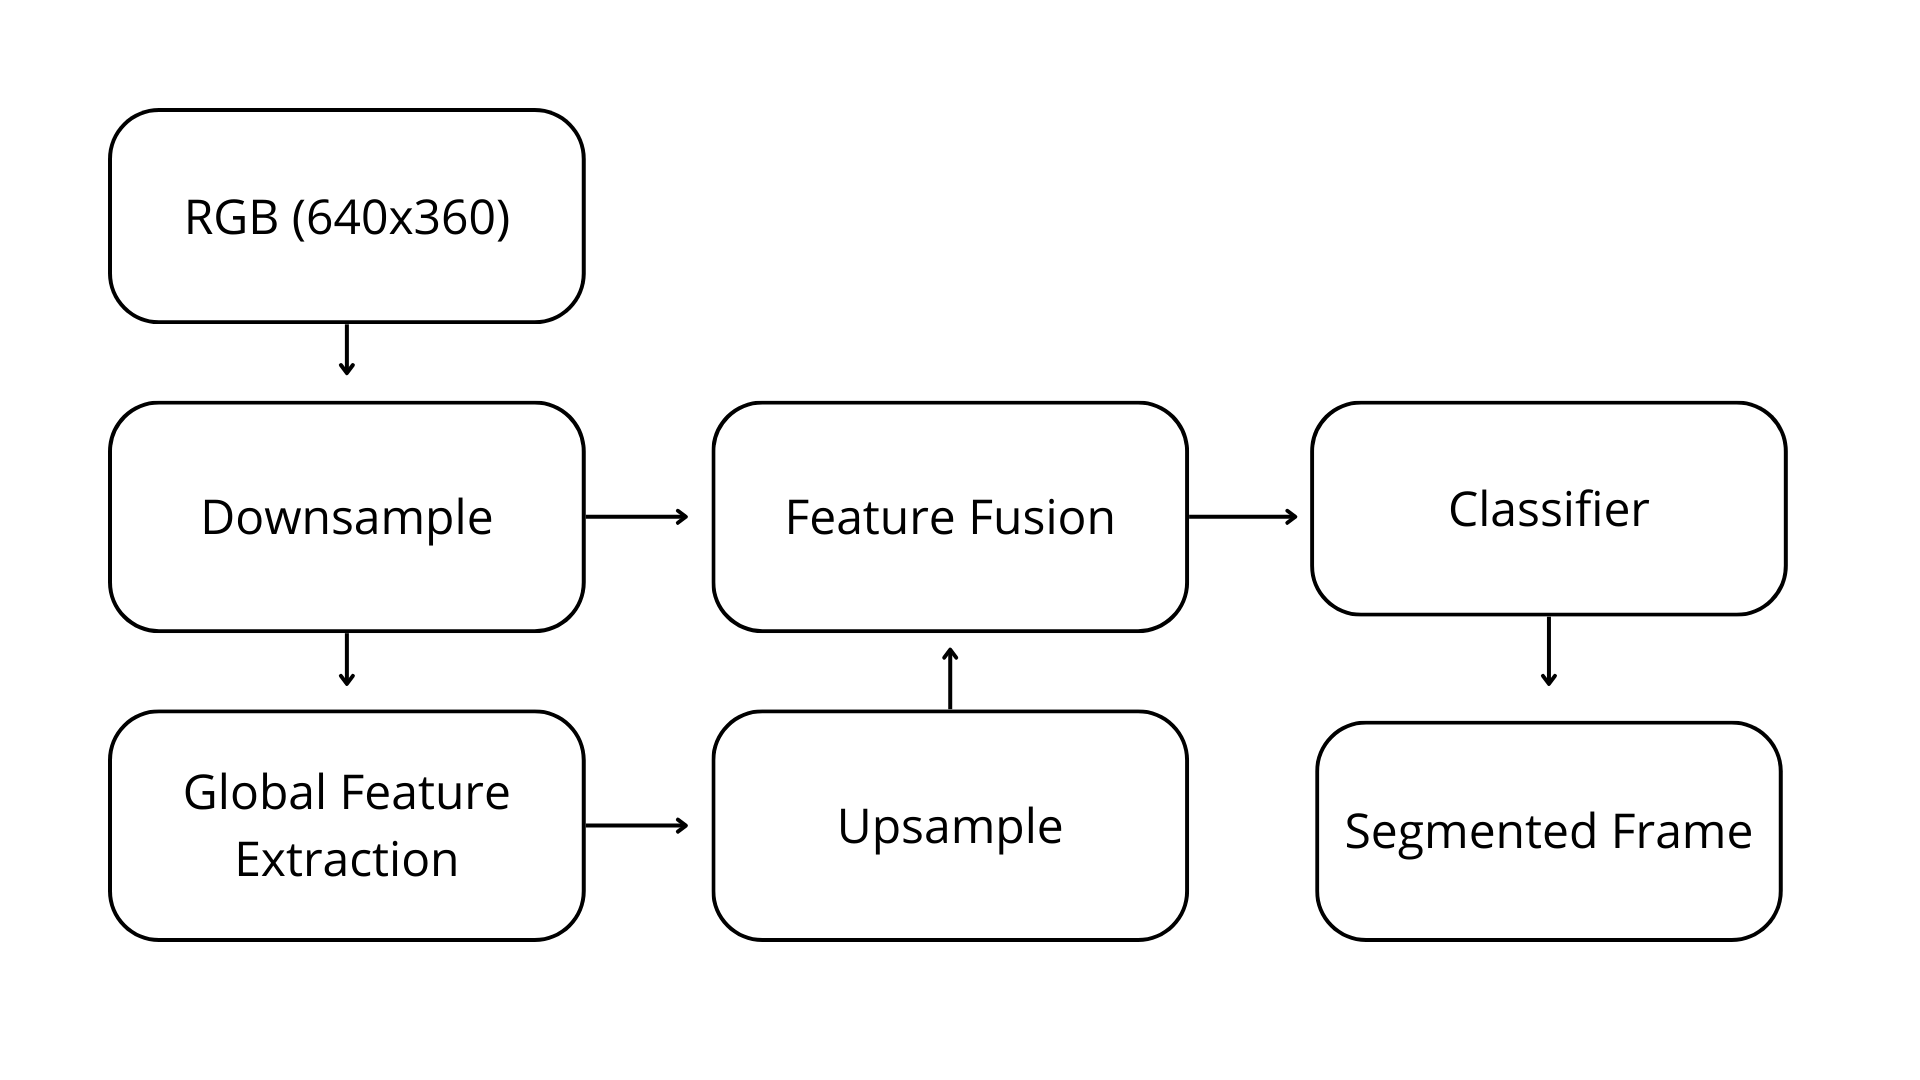
\includegraphics[width=\linewidth]{../konten/ml_sys.png}
	\caption{Block Diagram of the Machine Learning Architecture on Icar}
	\label{fig:ml_system}
\end{figure} 

From Figure \ref{fig:ml_system}, it is shown that the road detection system on Icar utilizes a machine learning architecture, specifically using Fast-SCNN \cite{ref_fast_scnn} as the core model. Its architecture differs in the convolution channels and pooling methods. The smaller convolution channels and the use of average pooling instead of pyramid pooling are intended to reduce computational load, making it suitable for real-time applications on Icar.

\subsubsection{Downsampling} 
In this step, the image captured by the stereo depth camera, originally a 3-channel image, is converted to 16 channels. This is achieved via three successive 3x3 convolution layers with a stride of 2: first converting 3→4 channels, then 4→8, and finally 8→16 channels. The resulting image is then split into two paths: one goes to global feature extraction, the other to feature fusion.

\subsubsection{Global Feature Extraction}
This stage performs a depthwise-separable convolution to extract features from the 16-channel image. This method is chosen for its computational efficiency. The result is a 24-channel image, which is passed on to the upsampling stage.

\subsubsection{Upsampling}
This step performs pooling using average pooling, which is lighter and faster compared to the pyramid pooling used in the original Fast-SCNN. A convolution then produces a 32-channel output, which is passed to feature fusion.

\subsubsection{Feature Fusion}
Here, outputs from the downsampling and global feature extraction stages are merged into a 48-channel image. Before merging, image dimensions are matched using bilinear interpolation. The merged result is passed to the classification stage.

\subsubsection{Classification}
In this final stage, the 48-channel image undergoes classification using ReLU, producing a 2-channel image indicating road and non-road areas. This image then proceeds to post processing.

\subsection{Pose and Orientation Correction System}
\begin{figure}[H]
	\centering
	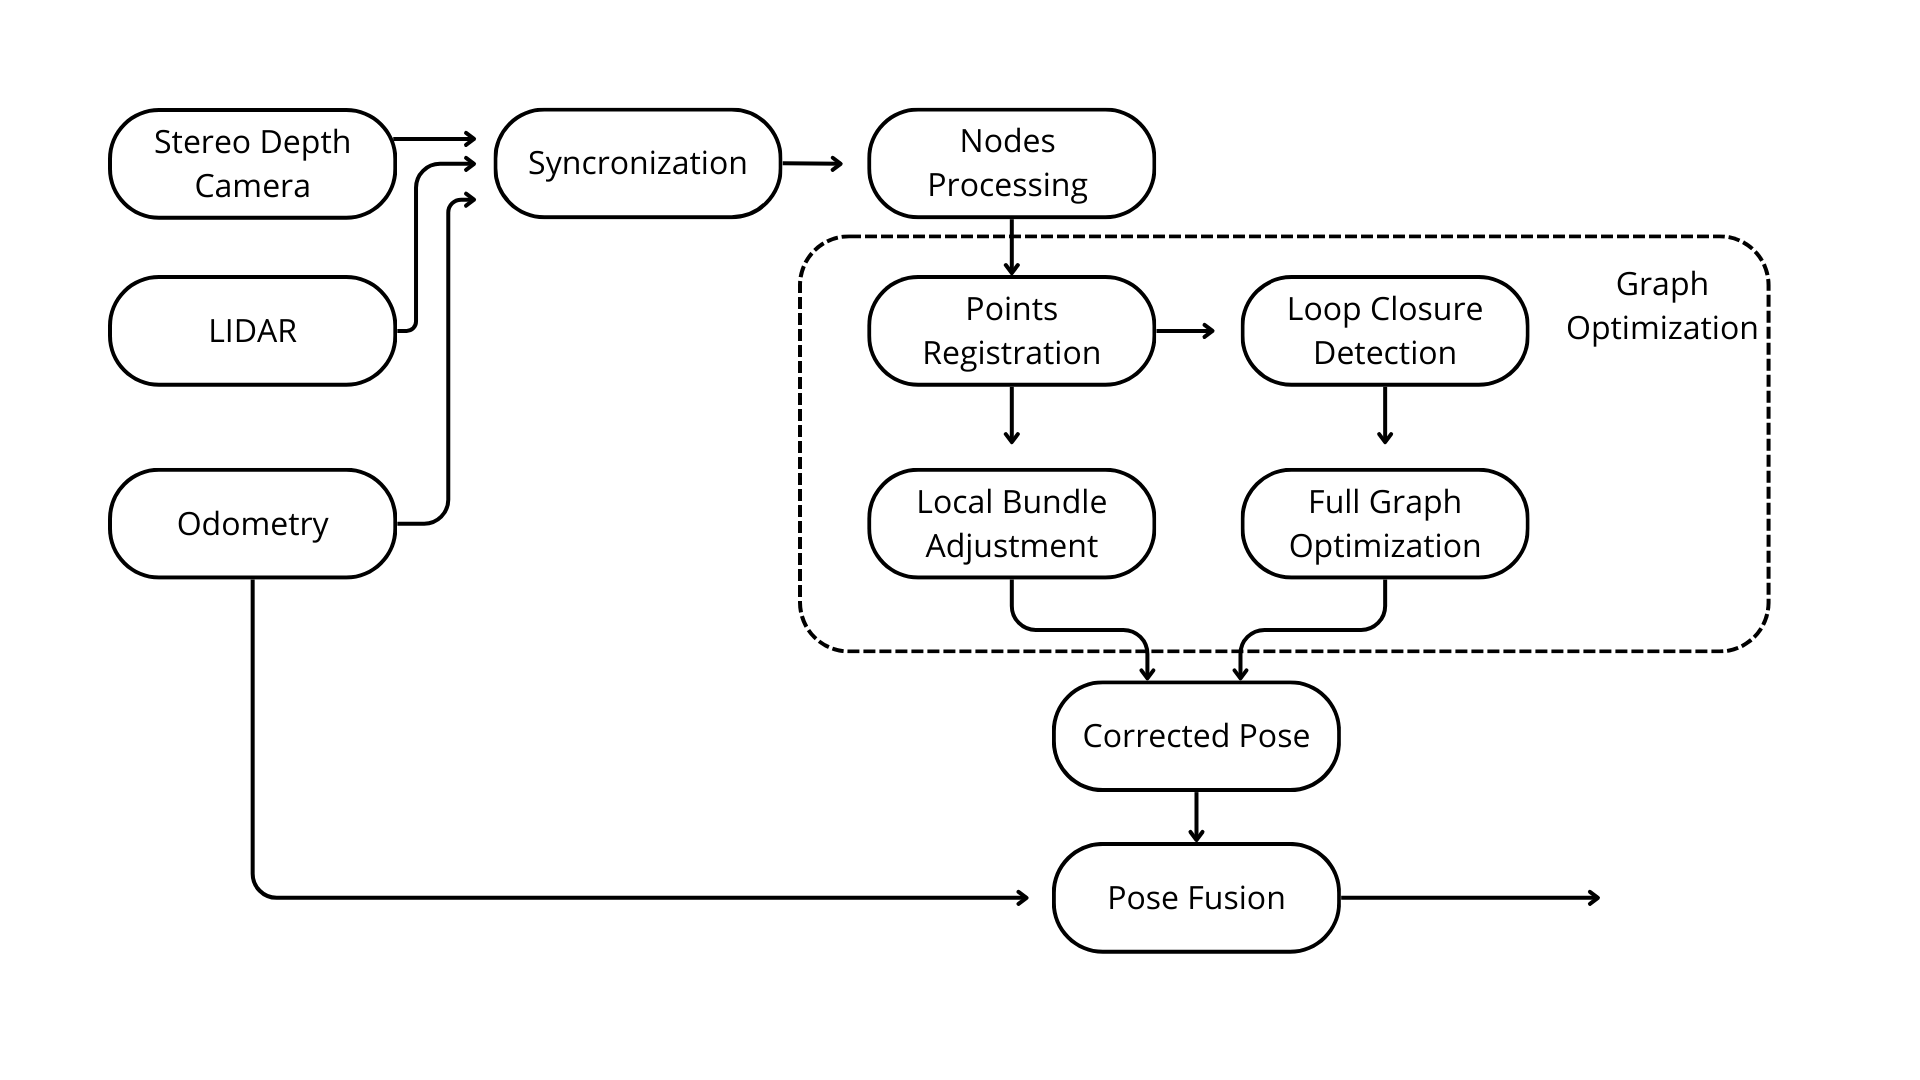
\includegraphics[width=\linewidth]{../konten/slam_sys3.png}
	\caption{Block Diagram of Pose and Orientation Correction System on Icar}
	\label{fig:slam_system}
\end{figure} 

From Figure \ref{fig:slam_system}, the pose correction system consists of four main processes: data synchronization, nodes processing, graph optimization, and pose fusion.

\subsubsection{Data Synchronization} 
This initial step synchronizes data from the stereo depth camera and odometry based on timestamps to ensure aligned data for further processing.

\subsubsection{Nodes Processing}
This initiates the graph optimization process. Nodes represent vehicle poses and keypoints from stereo depth camera and LIDAR. There are two modes:
- In mapping mode, new nodes are continuously added.
- In localization mode, existing nodes are used without adding new ones.

\subsubsection{Graph Optimization} 
This is the core component, using the GTSAM library. It starts with points registration using the Iterative Closest Point (ICP) algorithm to align point clouds, resulting in a transformation matrix.

Next are two procedures:
- Local bundle adjustment optimizes surrounding nodes using the transformation, based on the Levenberg-Marquardt algorithm.
- Loop closure finding that identifies revisited nodes. When a loop closure is found, a full graph optimization is performed, optimizing all nodes globally. 

\subsubsection{Pose Fusion} 
The final step combines poses from graph optimization and odometry using a Kalman Filter, resulting in more accurate pose estimation than using odometry alone. Using the differential data from Odometry (Wheel encoder and IMU) combined with estimated pose that coming from Graph Optimization, the system can correct the pose and orientation of Icar.

\subsection{Icar Navigation System with Road Detection and Graph-Based SLAM} 
\begin{figure}[H]
	\centering
	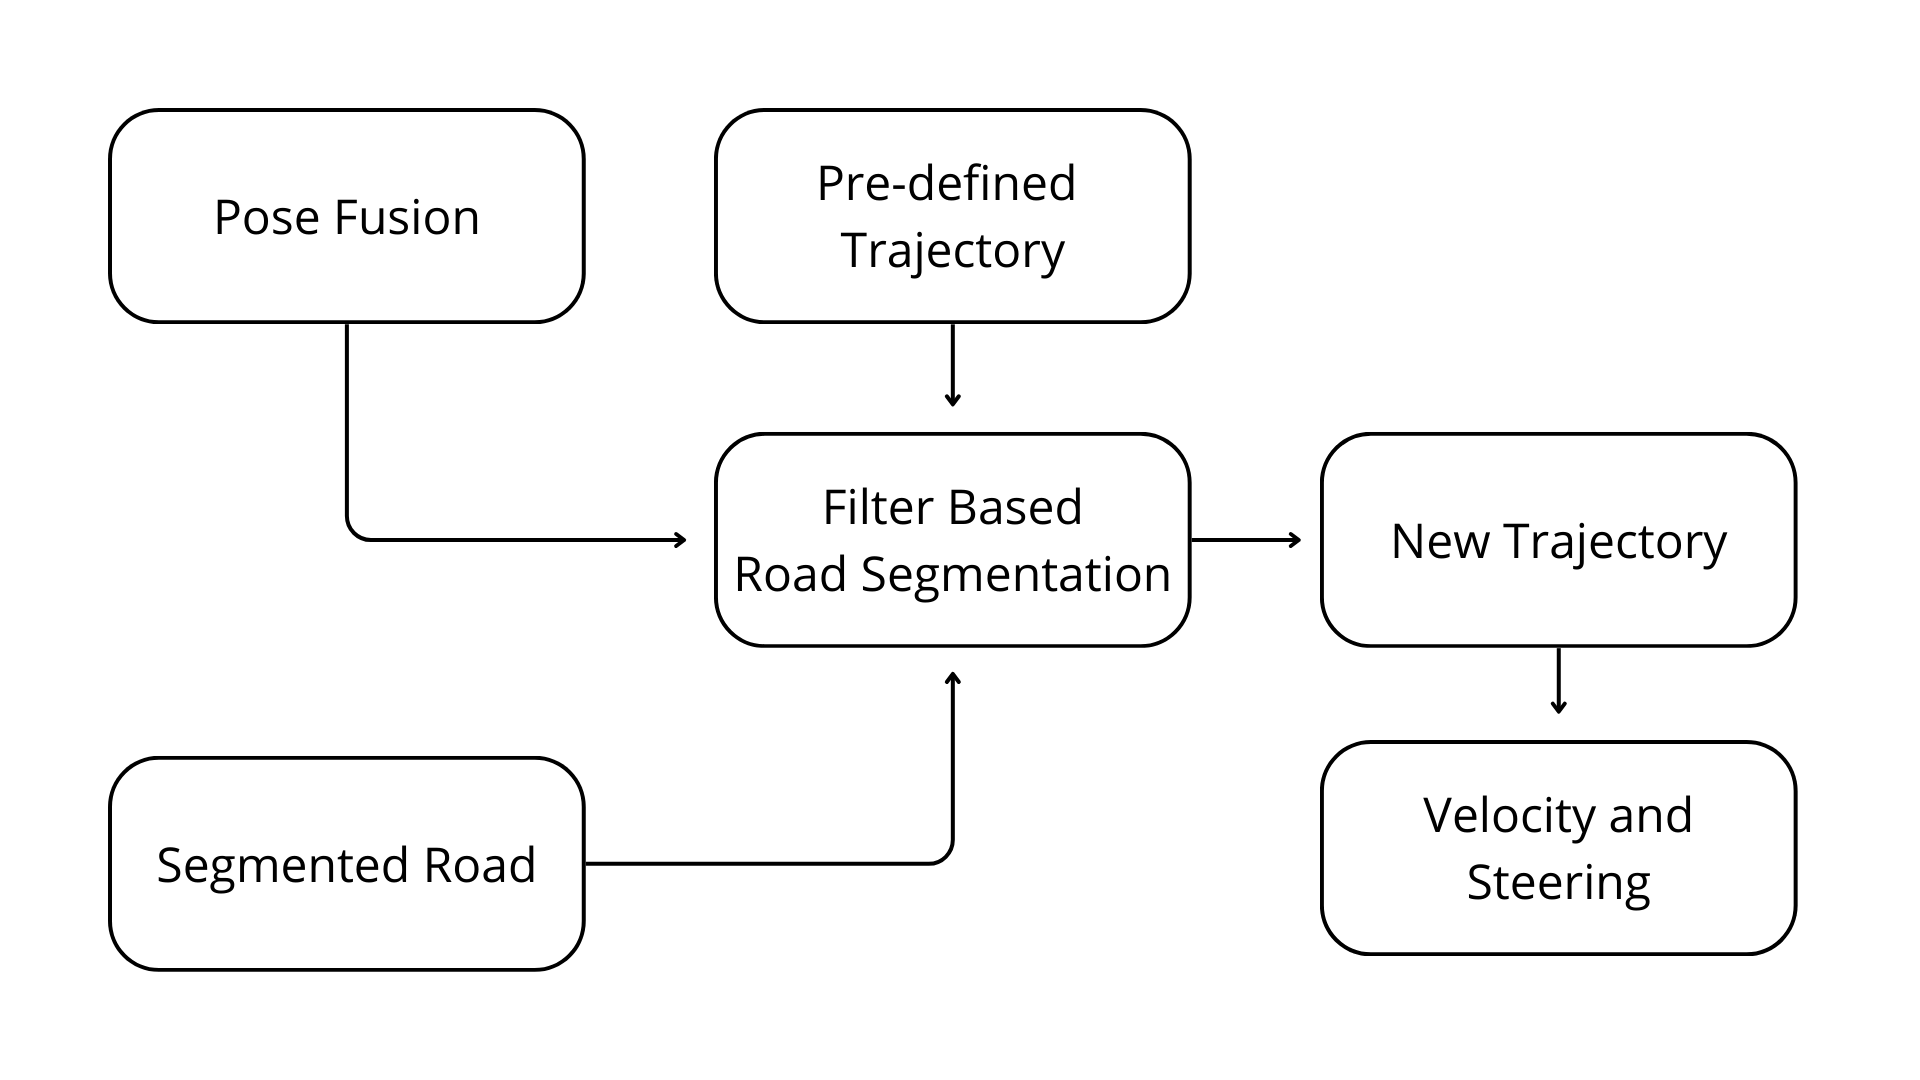
\includegraphics[width=\linewidth]{../konten/nav_new_sys3.png}
	\caption{Block Diagram of Icar Navigation System with Road Detection and Graph-Based SLAM}
	\label{fig:nav_new_system}
\end{figure} 

This diagram expands upon Figure \ref{fig:full_system_slam}, showing how the segmented road image from Figure \ref{fig:ml_system} and the pose data from Figure \ref{fig:slam_system} are integrated into a unified and improved navigation system.

\par  
The first step selects waypoints based on current pose (from graph-based SLAM) and the pre-defined trajectory. These waypoints are overlaid on the road segmentation image.

\par   
Next, a check is performed using a bitwise AND operation to determine if all waypoints lie within the road area. If so, the selected waypoints are used as the new trajectory.

\par  
If any waypoint lies outside the road, a new trajectory is generated using the image’s center of mass, converted into vehicle coordinates. A straight line is then created from the current position to the center of mass.

\par 
This new trajectory is then used for vehicle navigation. The vehicle follows it using the Bicycle Model as defined in Equation \ref{eq:bicycle_model_full} to calculate target speed and steering angle.


% Menamcement of realsensepilkan daftar pustaka dengan format IEEE
\bibliographystyle{IEEEtranN}
\bibliography{../ubah/pustaka.bib}

% Menyeimbangkan bagian akhir di kedua kolom
% \balance


\end{document}
